\documentclass{beamer}

%%%%%%%%%%%%%Solarized Theme%%%%%%%%%%%%%%%
\usecolortheme[dark,accent=cyan]{solarized}
\beamertemplatenavigationsymbolsempty
%%%%%Packages%%%%%
\usefonttheme{serif}
\usepackage[T1]{fontenc}
\usepackage[utf8]{inputenc}
\usepackage[english]{babel}
\usepackage{fontawesome}
\usepackage{minted}
\usepackage{soul}
\usepackage{ulem}
\usepackage{blkarray}
\usepackage{multirow}

\definecolor{DarkGray}{gray}{0.1}
\usemintedstyle{paraiso-dark}


\usepackage{graphicx}
\usepackage{hyperref}
\usepackage{colortbl, xcolor}
\usepackage{booktabs}
\usepackage{amsmath,amsthm, amssymb, latexsym}

\usepackage{tikz}
\usepackage{xcolor}
\usepackage{graphicx,multirow}
\definecolor{plain}{rgb}{93,93,93}
\usetikzlibrary{positioning,arrows}
\definecolor{applegreen}{rgb}{0.55, 0.71, 0.0}
\usetikzlibrary{decorations.pathreplacing, backgrounds, fit,}
\usetikzlibrary{calc,matrix}

\tikzstyle{background}=[solarizedRed, rectangle, draw, inner sep=1mm, thick,
           rounded corners=2mm]

\tikzset{
  treenode/.style = {align=center, inner sep=0pt, text centered,
    font=\sffamily},
  arn_n/.style = {treenode, circle, white, font=\sffamily\bfseries, draw=black, inner sep=-6pt,
    fill=black, text width=1.5em},% arbre rouge noir, noeud noir
  arn_r/.style = {treenode, circle, red, 
    text width=1.5em, very thick, inner sep=4pt},% arbre rouge noir, noeud rouge
  arn_x/.style = {treenode, rectangle, draw=black,
    minimum width=0.5em, minimum height=0.5em}% arbre rouge noir, nil
}

\usepackage{standalone}
\usepackage{siunitx}

\begin{document}

\begin{frame}
    \begin{center}
        \Large{\textcolor{orange}{Evolution of cooperation among individuals with limited payoff memory}} \\
        \vspace{.5cm}

        \vspace{1cm}
        \normalsize{ICSD 2022} \\
        \vspace{.5cm}
        \normalsize{Nikoleta Glynatsi, Christian Hilbe, Alex McAvoy}

    \end{center}
\end{frame}


\begin{frame}
    \begin{center}
    
\includegraphics[width=0.24\textwidth]{static/mpi.jpg}\hspace{8pt}
    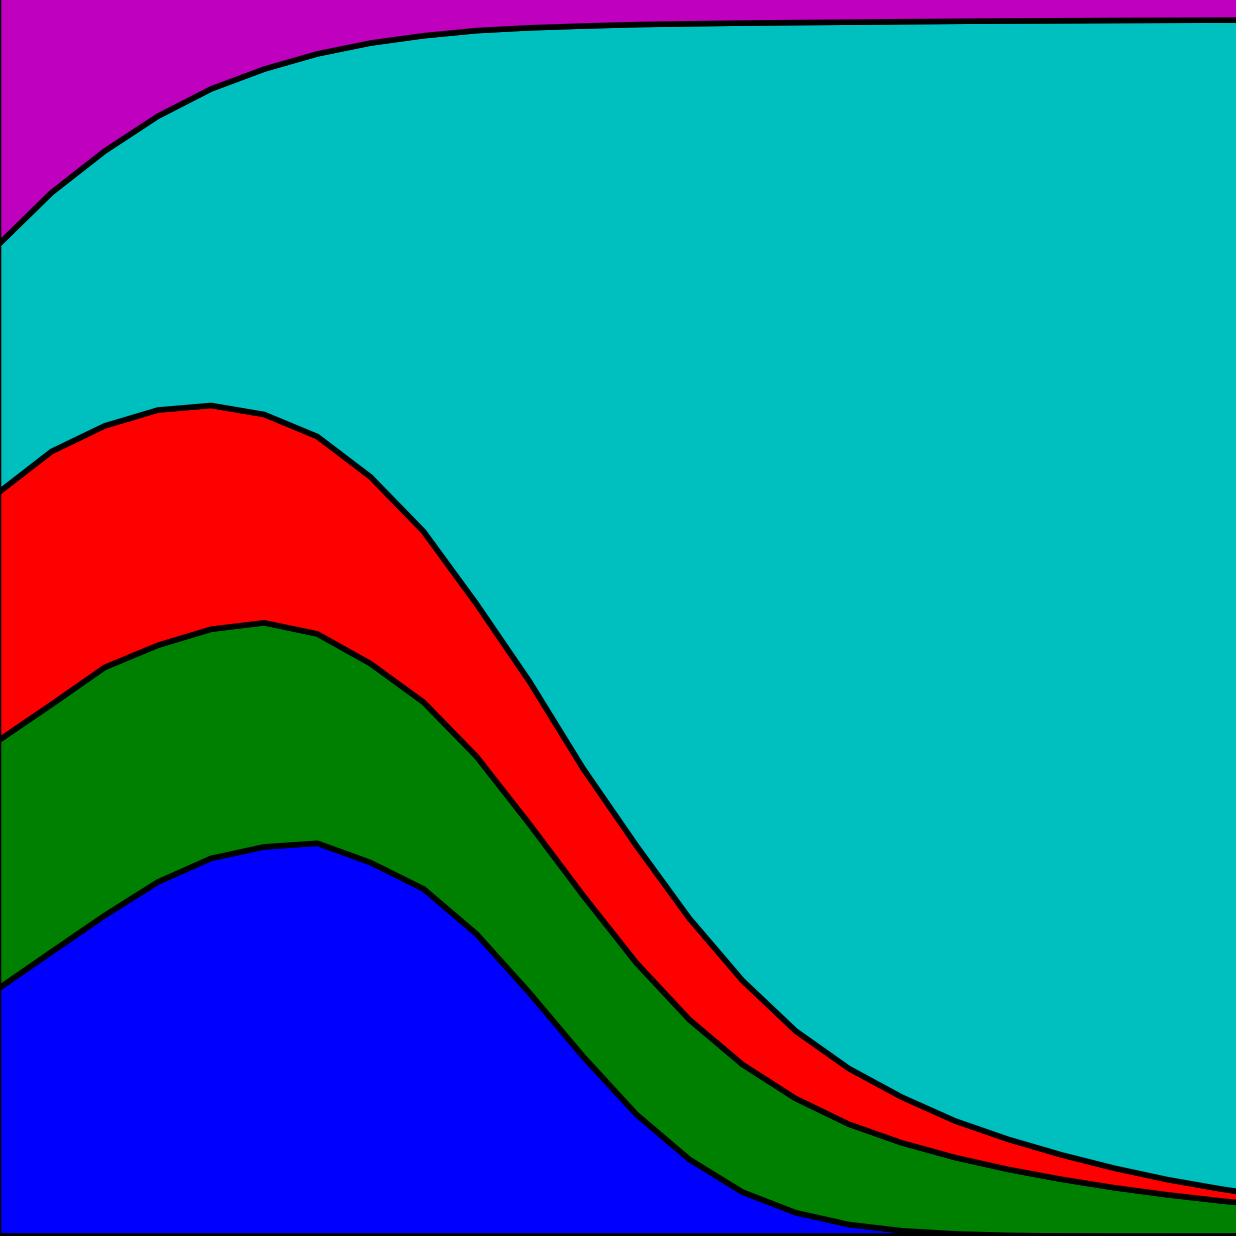
\includegraphics[width=0.24\textwidth]{static/axelrod-logo.png}
    
    % \vspace{8pt}

    % \includegraphics[width=0.24\textwidth]{static/joss.png}\hspace{8pt}
    % 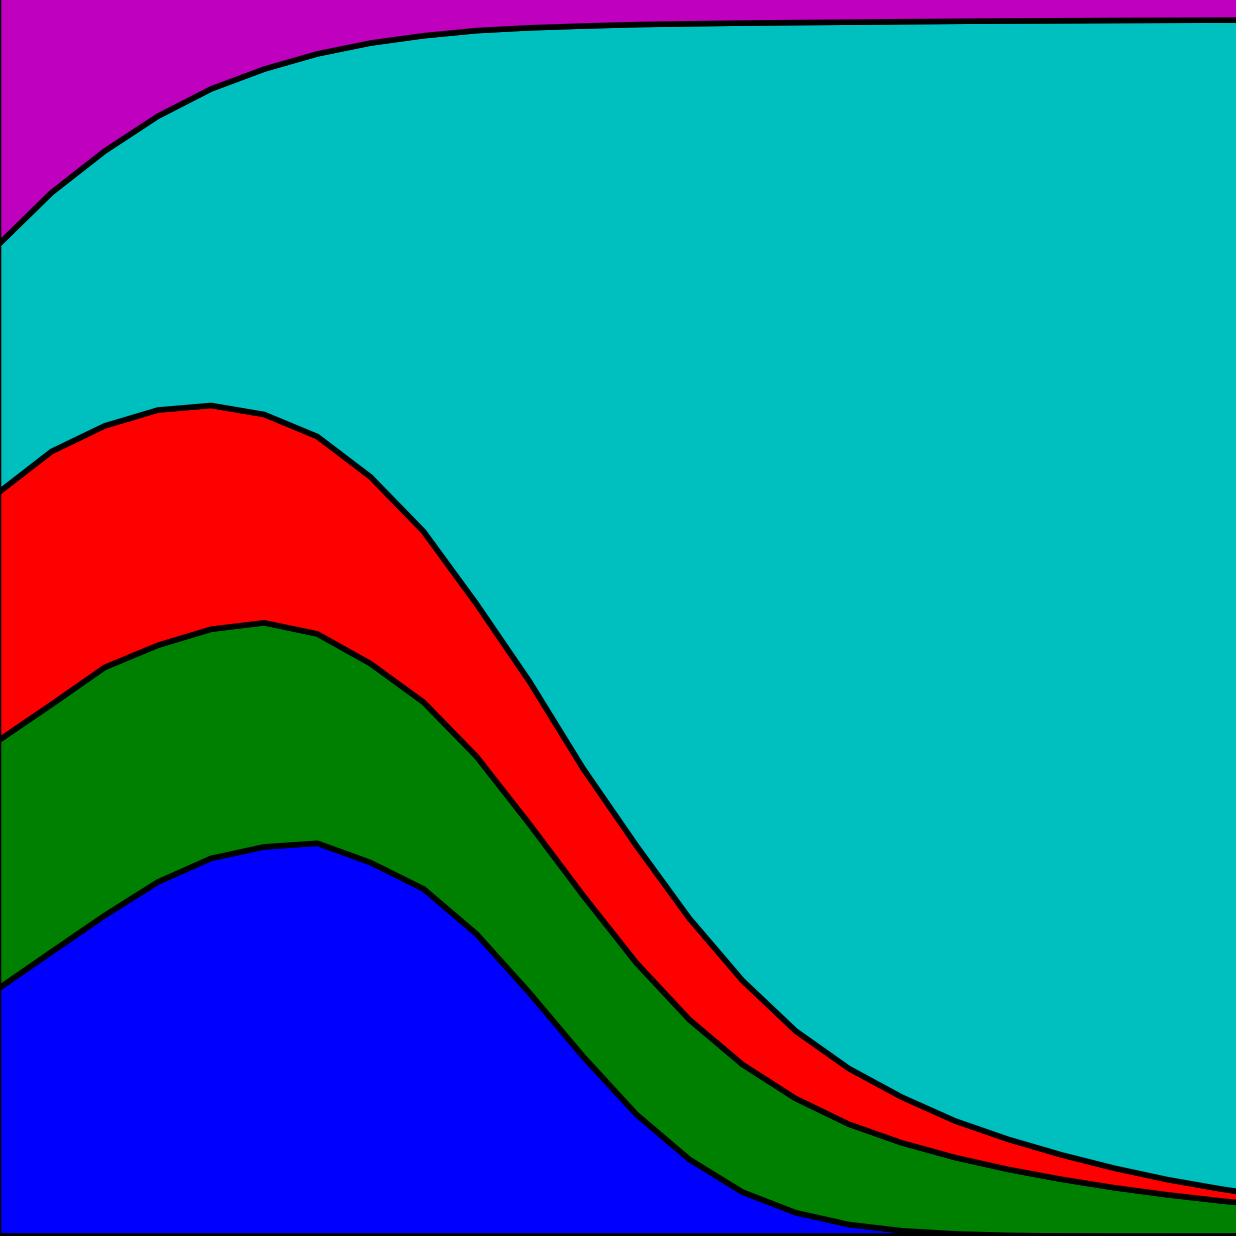
\includegraphics[width=0.24\textwidth]{static/axelrod-logo.png}

    \end{center}
\end{frame}

\begin{frame} \textbf{
    \begin{center}
    \Huge{
        \begin{equation*}
            \begin{blockarray}{c(cc)}
                 & b - c & -c \\
                 & b & 0 \\
            \end{blockarray}
        \end{equation*}}
    \end{center}}
\end{frame}

\begin{frame}
    \centering
    \Large{How do we model the evolution of cooperation?}
\end{frame}

\begin{frame}
    \centering
    \includestandalone[width=.65\textwidth]{static/pairwise_comparison_one}
\end{frame}

\begin{frame}
    \centering
    \includestandalone[width=.65\textwidth]{static/pairwise_comparison_two}
\end{frame}

\begin{frame}
    \centering
    \includestandalone[width=.65\textwidth]{static/pairwise_comparison_three}
\end{frame}

\begin{frame}
    \centering
    \includestandalone[width=.67\textwidth]{static/pairwise_comparison_four}
\end{frame}

\begin{frame}
    \centering
    \includestandalone[width=.65\textwidth]{static/pairwise_comparison_five}
\end{frame}

\begin{frame}
    \centering
    \Large{$$\rho = \frac{1}{1 \; + \; e^{\; - \; \beta (\pi _{{\rm A}}\; - \; \pi _{{\rm B}})}}$$}
\end{frame}

\begin{frame}
    \begin{center}
    
\includegraphics[width=0.15\textwidth]{static/magnifying_glass.png}\hspace{8pt}
    
\includegraphics[width=0.15\textwidth]{static/eyes.png}
    \end{center}
\end{frame}

\begin{frame}
    \centering
    \includestandalone[width=.65\textwidth]{static/game_stage}
\end{frame}

\begin{frame}
    \centering
    \Large{$\pi_A$ and $\pi_B$?}
\end{frame}

\begin{frame}
    \centering
    \includestandalone[width=.65\textwidth]{static/fitness_three}
\end{frame}

\begin{frame}
    \centering
    \includestandalone[width=.75\textwidth]{static/payoffs}
\end{frame}

% \begin{frame}
%     \centering
%     \includestandalone[width=.55\textwidth]{static/game_stage_payoffs}
% \end{frame}

\begin{frame}
    \centering
    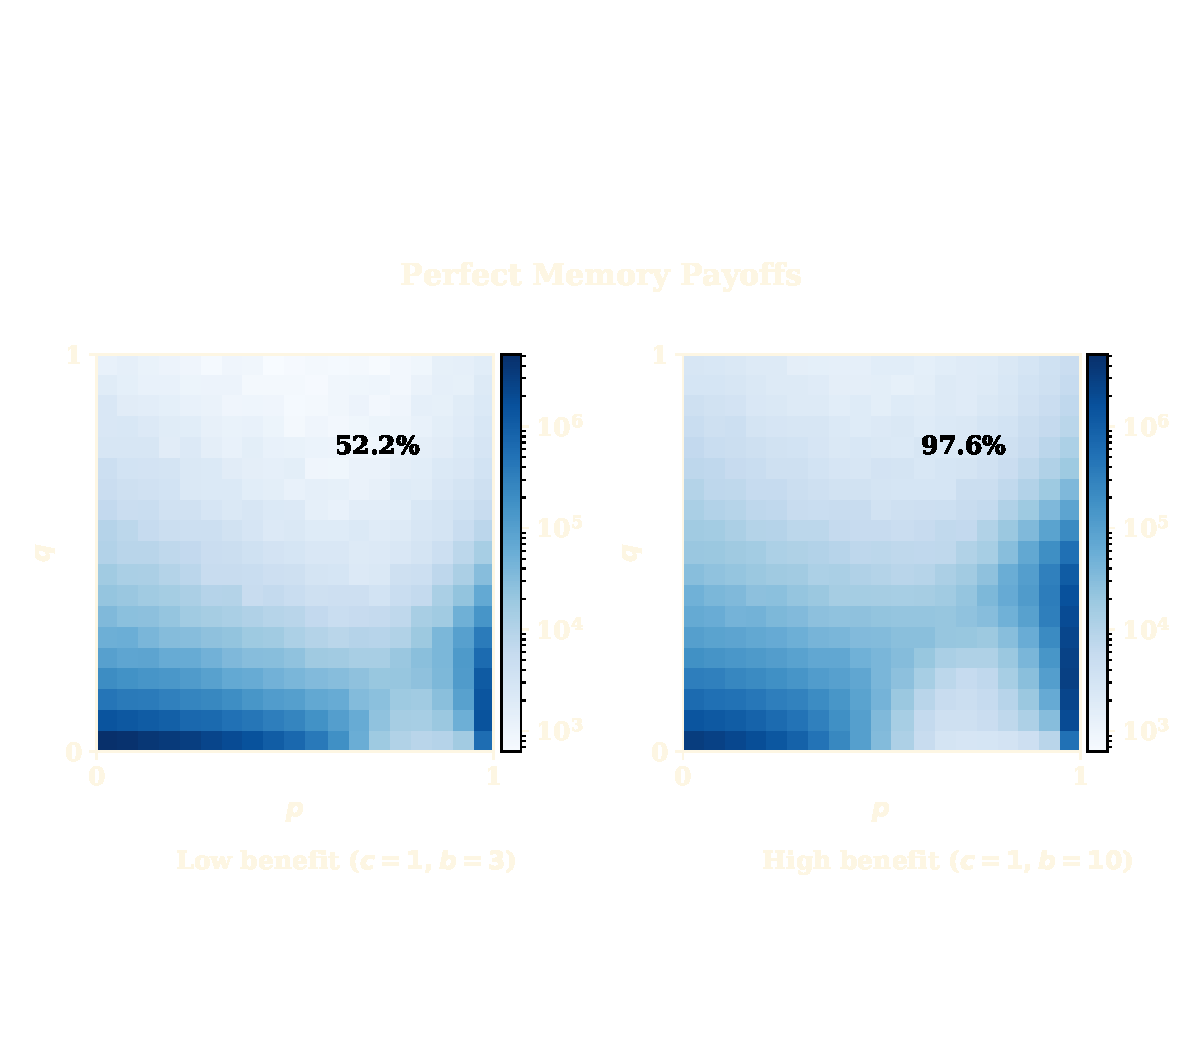
\includegraphics[width=\textwidth]{static/results_one.pdf}
\end{frame}

\begin{frame}
    \centering
    \includestandalone[width=\textwidth]{static/issue}
\end{frame}

\begin{frame}
    \centering
    \includestandalone[width=\textwidth]{static/solution}
\end{frame}

\begin{frame}
    \centering
    \includestandalone[width=.85\textwidth]{static/fitness_two}
\end{frame}

\begin{frame}
    \centering
    \includestandalone[width=.55\textwidth]{static/game_stage_payoffs_corrected}
\end{frame}

\begin{frame}
    \centering
    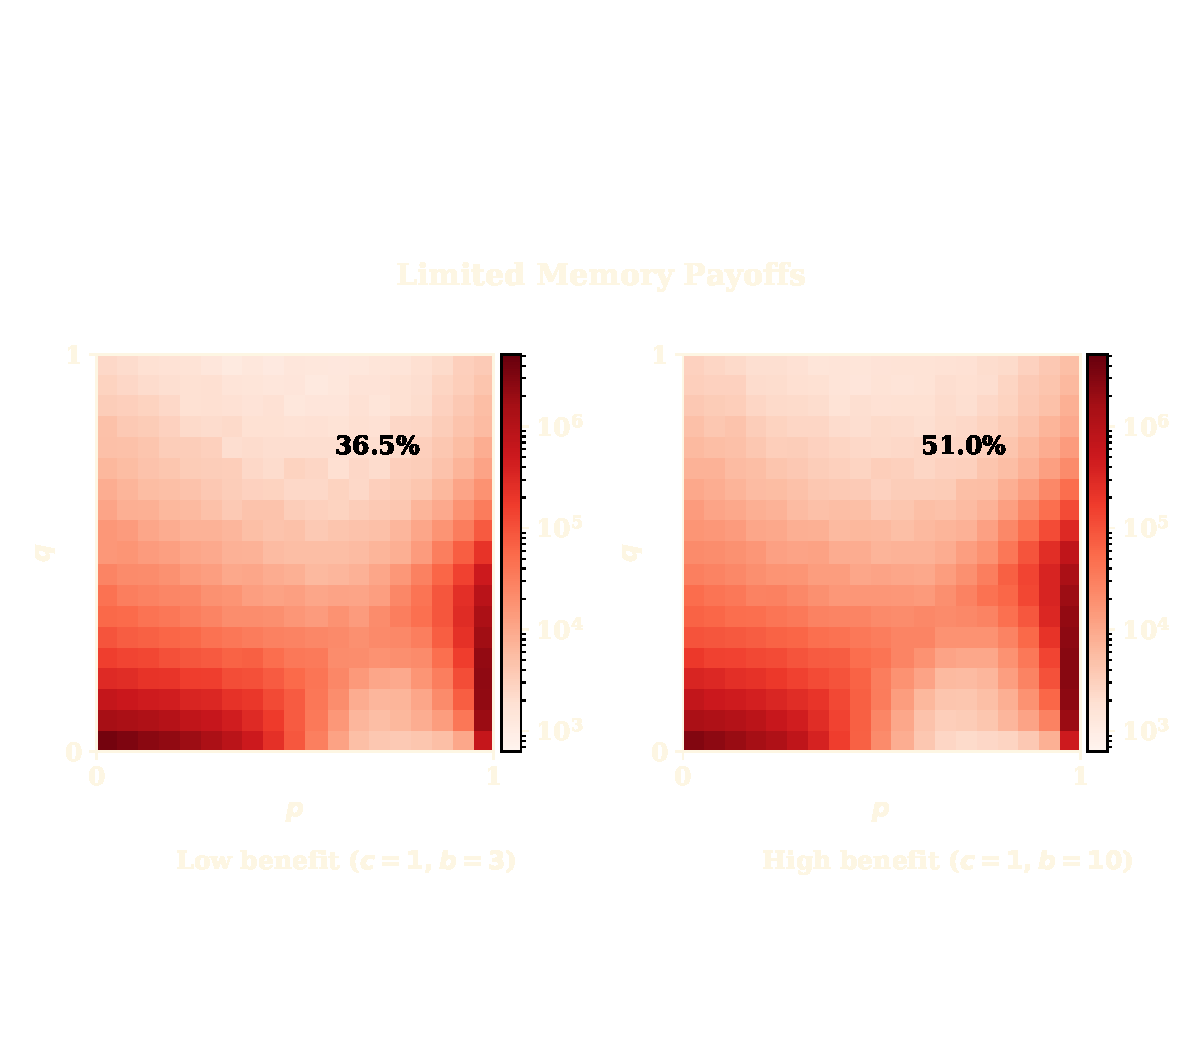
\includegraphics[width=\textwidth]{static/results_two.pdf}
\end{frame}

\begin{frame}
    \centering
    \includegraphics[width=\textwidth]{static/results_three.png}
\end{frame}

\begin{frame}
    \centering
    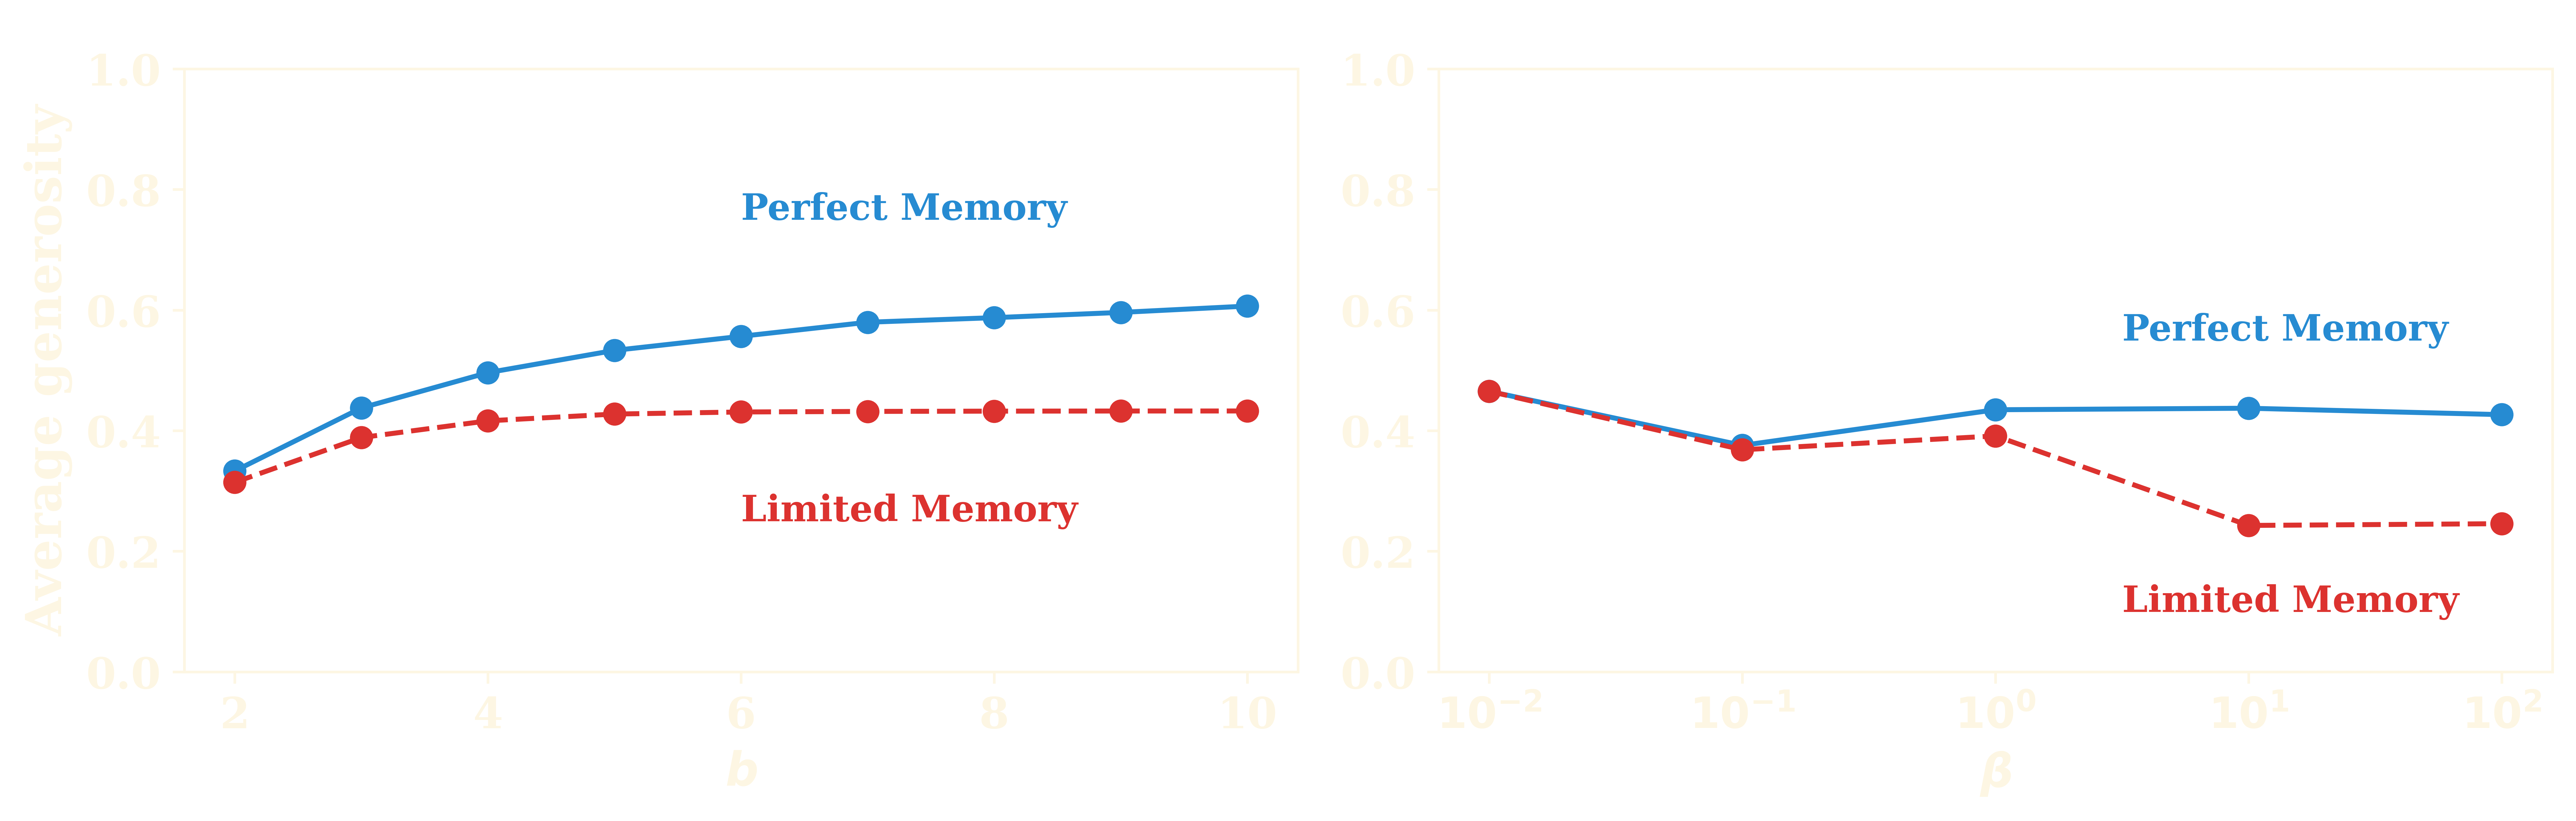
\includegraphics[width=\textwidth]{static/results_four.png}
\end{frame}

\begin{frame}
    \centering
    \includestandalone[width=.5\textwidth]{static/further}
\end{frame}

\begin{frame}
    \centering
    \includegraphics[width=\textwidth]{static/results_five.png}
\end{frame}

\begin{frame}
    \begin{center}
    \faTwitter \ @NikoletaGlyn \\
    \faTwitter \ @chilbe3 \\
    \vspace{1cm}

    \faGithub \ Nikoleta - v3 \\
    http://web.evolbio.mpg.de/social-behaviour/ \\
    \vspace{1cm}

    
\includegraphics[width=.3\textwidth]{static/erc.png}
    \end{center}
\end{frame}

\end{document}